% This is LLNCS.DEM the demonstration file of
% the LaTeX macro package from Springer-Verlag
% for Lecture Notes in Computer Science,
% version 2.4 for LaTeX2e as of 16. April 2010
%
\documentclass{llncs}
%
\usepackage{makeidx}  % allows for indexgeneration
\usepackage{graphicx}
\usepackage{url}
\usepackage[utf8]{inputenc}

\hyphenation{a-so-cia-das}
\hyphenation{re-fe-ren-cias}
\hyphenation{herra-mien-tas}

\setcounter{tocdepth}{2}
%
\begin{document}
\frontmatter
\pagestyle{headings}  % switches on printing of running heads

\addtocmark[2]{Recuperación de Información Geográfica}
\mainmatter              % start of the contributions
%
\title{Recuperación de Información Geográfica}
%
\titlerunning{Recuperación de Información Geográfica}  % abbreviated title (for running head)
%                                     also used for the TOC unless
%                                     \toctitle is used
%
\author{Jorge J. Morgado Vega\inst{1} \and Roberto García Rodrígez\inst{1}}
%
% \authorrunning{Ivar Ekeland et al.} % abbreviated author list (for running head)
%
%%%% list of authors for the TOC (use if author list has to be modified)
\tocauthor{Jorge J. Morgado Vega y Roberto García Rodrígez}
%
\institute{Universidad de la Habana, La Habana, Cuba}

\maketitle              % typeset the title of the contribution

\renewcommand\abstractname{Resúmen.}
\renewcommand\keywordname{{\bf Palabras Claves:}}
\begin{abstract}
	Uno de los subcampos de la Recuperación de Información (RI) es la
	Recueración de Información Geográfica (RIG). Los sistemas de RIG son de
	gran utilidad en diferentes esferas de la sociedad, a nivel gubernamental,
	empresarial, personal, etc. En este trabajo se realizará un análisis del
	estado del arte de la RIG. Se abordarán algunas de las arquitecturas
	implementadas, la evaluación de estos sistemas, sus aplicaciones, los
	beneficios y limitantes así como desafíos futuros en este campo
	investigativo.
\keywords{recuperación de información, información geográfica}
\end{abstract}
\renewcommand\abstractname{Abstract.}
\renewcommand\keywordname{{\bf Keywords:}}
\begin{abstract}
	One of the subfields of Information Retrieval (IR) is Geographic Information
	Retrieval (GIR). GIR systems are very useful in different spheres of society,
	government, business, personal, etc. In this work, an analysis of the state of
	the art of RIG will be carried out. Some of the implemented architectures, the
	evaluation of these systems, their applications, the benefits and limitations
	as well as future challenges in this research field will be addressed.
\keywords{information retrieval, geographic information}
\end{abstract}
%

\tableofcontents
\clearpage
\section{Características del Problema}\label{sec:prob-charact}

Los Sistemas de Recuperación de Información (SRI) tienen una amplia gama de
variantes, surgidas a partir de las distintas necesidades de la vida cotidiana
y otras problemáticas que han aparecido a lo largo del desarrollo de la
humanidad. A medida que las necesidades de las personas van evolucionando así
lo hacen los SRI. Es por ello que cada vez es más necesario que estos sistemas
sean más rápidos y eficaces.

Uno de los subcampos de los SRI es la Recuperación de Información Geográfica
(RIG). La RIG surge de la unión de de los SRI y los Sistemas de Información
Geográficos (SIG), los cuales se enfocan en el desarrollo y uso de teorías,
métodos, tecnologías y datos para comprender los procesos geográficos,
relaciones y patrones \cite{chang2016}.

Los sistemas de RIG se emplean en la búsqueda local móvil, en la web y en
documentos empresariales. Estos sistemas que combinan consultas tradicionales
basadas en texto con consultas de ubicación, como mapas o nombres de lugares.
Son técnicas para construir un sistema de aplicación que pueda indexar,
consultar, recuperar y navegar por la información georreferenciada. El objetivo
de los sistemas de RIG es comprender mejor el conocimiento geográfico contenido
en la web, documentos y consultas de los usuarios, y proporcionar una respuesta
más satisfactoria a sus necesidades.

Una de las características propias de los sistemas de RIG es que en muchas
ocasiones la información obtenida puede ser visualizada de diferentes formas
(comúnmente en mapas). Esto permite a los usuarios tener una mejor
percepción de la información y una mejor comprensión de la misma.

Varios son los otros campos científicos que están presentes en los sistemas de
RIG: el procesamiento de lenguaje natural para la comprensión de textos no
estructurados y en las búsquedas que realizan los usuarios; la lingüística en
el análisis de documentos, búsquedas o datos de forma general que se encuentran
en otros idiomas; entre muchos otros.

En este trabajo se muestran los resultados de una investigación sobre el estado
del arte y uso de los Sistemas de Recuperación de Información Geográfica. El
mismo está estructurado de la siguiente forma: en la Sección \ref{sec:arch} se
mostrará la arquitectura de un sistema de RIG básico así como alguna de las
implementaciones que existen; en la Sección \ref{sec:eval} se analizará la
evaluación de estos sistemas; en la Sección \ref{sec:appl} se describirán las
diversas aplicaciones de los sistemas de RIG; en la sección
\ref{sec:pros-and-cons} se mostrarán los principales beneficios y limitantes
que existen al usar un sistema de RIG; y en la Sección \ref{sec:chall} se
describirán los retos que se presentan en el desarrollo de los sistemas de RIG
en la actualidad.

\newpage

\section{Arquitecturas Propuestas}\label{sec:arch}

Muchos son los sistemas de recuperación de información geográfica que se han
propuesto a lo largo del tiempo. En las siguientes secciones se analizará
tanto la arquitectura básica de estos sistemas así como algunas de las
propuestas más avanzadas.

\subsection{Arquitectura Básica}\label{sec:archbas}

Como se puede apreciar en la Figura \ref{fig:archbas}, la arquitectura básica
de un sistema de RIG consta de 3 estapas principales: adquisición de de datos,
indexado y finalmente, la búsqueda o recuperación de información. En la primera
etapa se utilizan \emph{crawlers} enfocados directamente a extraer información
geográfica de la web. Muchas de las fuentes no tienen los datos de forma
estructurada, es por ello que en la segunda etapa mucha de la información es
analizada y parseada. En esta estapa es donde la información se guarda en la
base de datos y es indexada. En la tercera etapa al realizar la búsqueda de la
información, la misma pasa por un proceso de \emph{ranking} o evaluación. Esto
permite que se pueda encontrar la información más relevante de una forma más
eficiente.

\begin{figure}[htb]%
	\begin{center}
		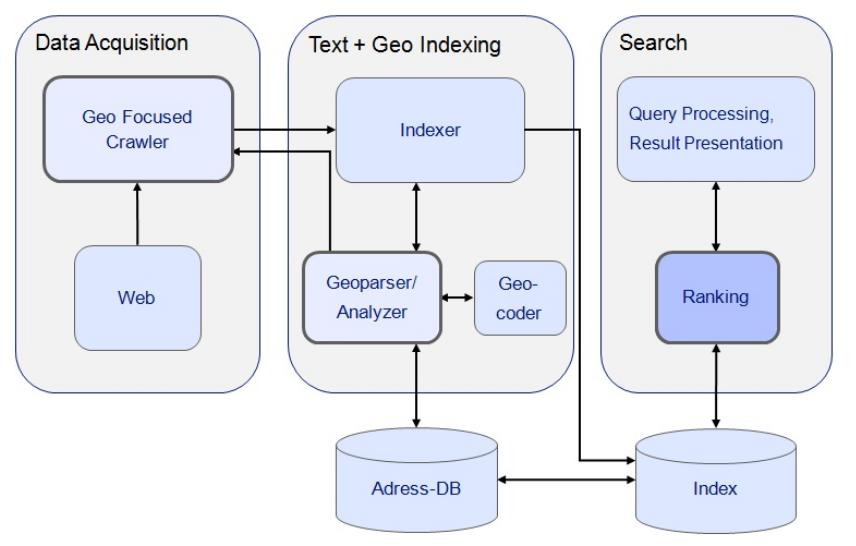
\includegraphics[width=0.6\textwidth]{basic_arch.jpg}
	\end{center}
	\caption{Arquitectura básica de un sistema de RIG \cite{cai2011}}
	\label{fig:archbas}
\end{figure}

\newpage

\subsection{SPIRIT}\label{sec:archspirit}

En esta propuesta el trabajo de \cite{purves2007} describe el diseño,
implementación y evaluación de un motor de búsqueda de información geográfica
el cual es capaz de realizar búsquedas en forma de tripletas: tema - relación
espacial - locación. Como se puede ver en la Figura \ref{fig:archspirit}, a los
documentos, además de ser indexados y almacenados en una base de datos, también
se les agrega un \emph{footprint} lo cual permite que se pueda identificar y
relacionar de forma más precisa la información.

\begin{figure}[htb]%
	\begin{center}
		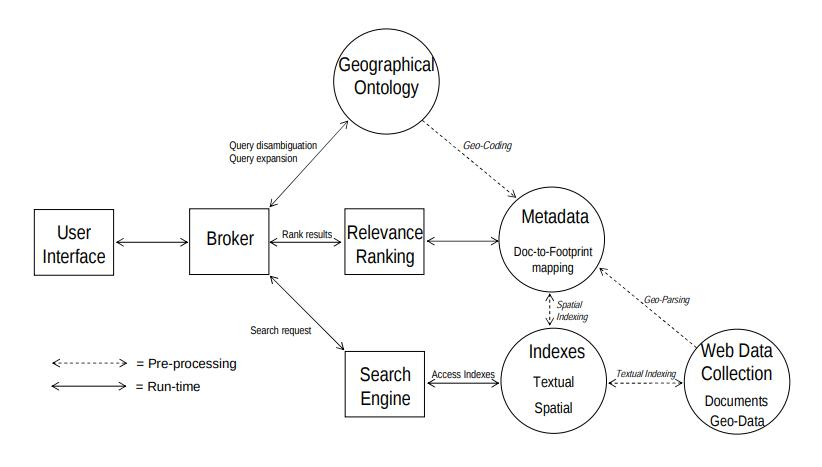
\includegraphics[width=0.6\textwidth]{spirit_arch.jpg}
	\end{center}
	\caption{Arquitectura de SPIRIT \cite{purves2007}}
	\label{fig:archspirit}
\end{figure}

En este sistema se aplicaron métodos para la búsqueda y exploración de los
resultados los cuales se evalúan en cuanto a su relevancia teniendo en cuenta
la temática y además la relación espacial de los mismos. Se hace uso también de
ontologías geográficas para la desambiguación de las búsquedas hechas por los
usuarios. Se muestran además dos formas de indexar la información: textual y
espacial. La primera forma de indexar (textual) se realiza directamente del
conjunto de documentos, la segunda forma (espacial) se puede apreciar en la
Figura \ref{fig:archspirit} que se realiza utilizando los metadatos agregados a
los documentos.

\newpage

\subsection{GeoUJA}\label{sec:archgeouja}

GeoUJA \cite{perea2007} es un sistema de RIG presentado por un grupo de la
Universidad de Ja'en en el evento GeoCLEF 2007. La arquitectura de este sistema
se basa en cinco módulos (o subsistemas) principales como se puede apreciar en
la Figura \ref{fig:archgeouja}. Los módulos son: subsistema de recuperación de
información, subsistema de traducción, subsistema de búsqueda de relaciones
geográficas, subsistema de reconocimiento de nombres de entidades y subsistema
de validación.

\begin{figure}[htb]%
	\begin{center}
		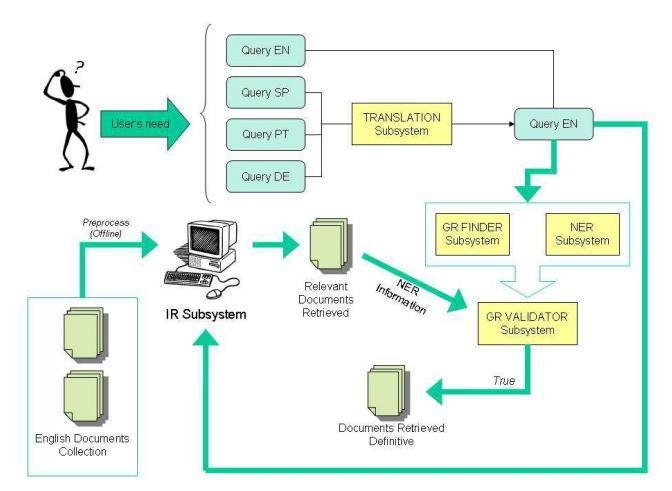
\includegraphics[width=0.6\textwidth]{geouja_arch.jpg}
	\end{center}
	\caption{Arquitectura de GeoUJA \cite{perea2007}}
	\label{fig:archgeouja}
\end{figure}

Primeramente el usuario ingresa una búsqueda (en cuatro posibles idiomas) la
cual, en caso de ser necesario, se traduce al inglés utilizando el susbsistema
de traducción, y se envía al subsistema de recuperación de información para
extraer los documentos relevantes. Esta búsqueda es también procesada por los
subsistemas de búsqueda de relaciones geográficas y reconocimiento de nombres de
entidades. Luego de este preprocesamiento, y en conjunto con los documentos
relvantes extraídos previamente, se realiza un validación de los mismos y se
devuelve al usuario un conjunto de documentos que el sistema en general
clasifica como relevantes.

\newpage

\subsection{GeoFinder}\label{sec:archgeofinder}

Otra arquitectura interesante a presentar es la que propone GeoFinder
\cite{bordogna2012}. En la misma se divide el proceso en dos módulos principales
como se puede apreciar en la Figura \ref{fig:archgeofinder}. El primer módulo es
el encargado de indexar los documentos. En este es donde se realiza la
\emph{estructuración} de los documentos (\emph{geo-indexing}) y se almacenan.
En el segundo módulo se realiza la búsqueda de la información.

\begin{figure}[htb]%
	\begin{center}
		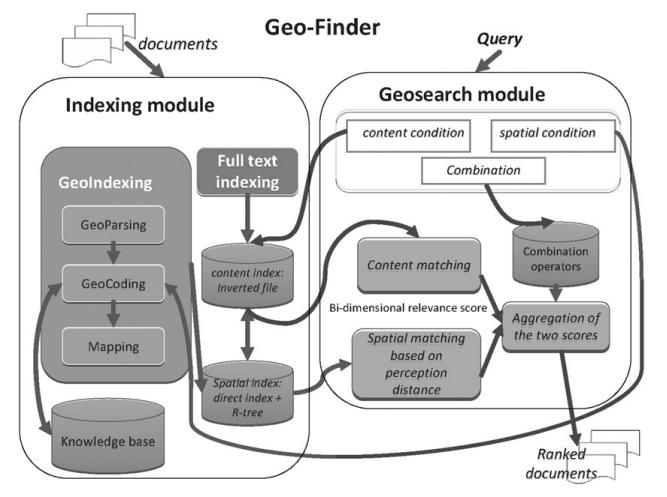
\includegraphics[width=0.6\textwidth]{geofinder_arch.jpg}
	\end{center}
	\caption{Arquitectura de GeoFinder \cite{bordogna2012}}
	\label{fig:archgeofinder}
\end{figure}

Al realizar una búsqueda, la misma se utiliza para consultar documentos
relacionados por el contenido y documentos relacionados espacialmente. Luego,
los documentos se evalúan teniendo en cuenta estas dos formas antes mencionadas
(contenido y espacio). Finalmente considerando ambas métricas los
resultados se combinan para extraer la mejor selección de documentos.

\clearpage

\section{Evaluación del Sistema}\label{sec:eval}

Los sistemas RIG, como cualquier otro sistema, se pueden someter a evaluación.
Es proceso es bastante parecido a los empleados en los SRI estándar, variando
solo algunos pasos específicos que el propio sistema impone dada las
características del mismo y del problema que pretende resolver (como por
ejemplo la detección de entidades geográficas) \cite{kornai2005}.

Paralelamente al desarrollo de estos sistemas, surge un amplio campo de
trabajo dedicado específicamente a la determinación de medidas que permitan
valorar su efectividad. Un repaso exhaustivo de la bibliografía especializada
permite identificar varios grupos de evaluaciones: las basadas en la
relevancia de los documentos, las basadas en los usuarios y un tercer grupo
de medidas alternativas a la realización de los juicios de relevancia, que
pretende evitar la afectación de estos juicios por las dosis de subjetividad que
poseen de forma inherente.

Los primeros estudios de evaluación de los SRI datan casi del surgimiento de
los mismos, siendo estos los pioneros de la evaluación de los sistemas, los
cuales sirvieron de base para la creación de futuros métodos y análisis que
se fueron transformando a través del tiempo y adaptándose a los nuevos
sistemas que fueron apareciendo. Estos estudios son Cranfield,
MEDLARS o SMART \cite{bors2000}.

Aunque la propia naturaleza del los sistemas de RIG difieran en ciertos aspectos
de los SRI estándar, como fue antes mencionado, la mayoría de los
métodos de evaluación empleados son también de uso estándar, o sea, la
aplicación de estos en los SRI clásicos han sido extendidos a los
demás modelos, siendo cada vez más confiables y de amplio uso en la actualidad.

\subsection{Método Cranfield}\label{sec:Cranfield}

Es uno de los primeros métodos de evaluación, su uso se ha estandarizado 
siendo hoy en día ampliamente usado en casi todos los sistemas como la base de
modelos más complejos \cite{hosseini2013}.

Evalúa la eficacia del sistema de recuperación de información según la
dimensión temática del documento y las consultas. Es un sistema de evaluación
donde se proporcionaba un objeto de estudio, una metodología de investigación
científica y un lenguaje terminológico.

Los autores determinaron la relevancia de los documentos en relación
con las preguntas formuladas a través de una escala formada por cuatro niveles
en detrimento de las escalas binarias (relevante \emph{vs} no relevante).
Estas categorías son las siguientes: 

\begin{enumerate}
    \item Documentos recuperados y relevantes.
    \item Documentos recuperados y no relevantes (ruido documental).
    \item Documentos no recuperados y relevantes (silencio documental).
    \item Documentos no recuperados y no relevantes. 
\end{enumerate}

\subsection{GeoCLEF}\label{sec:GeoCLEF}

GeoCLEF (\emph{Geographical CLEF}) es un marco de evaluación para la RIG que
pertenece al foro internacional \emph{Cross Language Evaluation Forum} (CLEF).
Fue una colaboración esfuerzo de los grupos de investigación de la Universidad
de California, Berkeley y la Universidad de Sheffield \cite{gey2005,kornai2005}.

El objetivo de GeoCLEF es proporcionar el marco de trabajo necesario para la
evaluación de estos sistemas de RIG en búsquedas de información, teniendo en
cuenta aspectos geo-referenciales y multilingües. Este evento se efectuó, en un
principio, como una prueba piloto para evaluar la recuperación de documentos
multilingües con énfasis en la búsqueda geográfica.

La colección de prueba de GeoCLEF crece en 25 temas cada año. Esto generalmente
se considera el tamaño mínimo de la colección de pruebas para producir
resultados confiables. Con estos temas se realizan pruebas estadísticas y
análisis adicionales para evaluar la validez de los resultados obtenidos.

\newpage

\section{Aplicaciones}\label{sec:appl}

Las aplicaciones de estos sistemas cada vez son más frecuentes, en ámbitos
tanto cotidianos como científicos. Hoy en día, muchos de los problemas
resueltos están orientados espacialmente, lo que significa que cada vez más
personas necesitan utilizar información espacial, acceso rápido a estos medios,
softwares y aplicaciones fáciles de usar (\emph{user friendly} en inglés), que no
requieran de conocimientos específicos ni formación especial. A continuación
se presentan algunas aplicaciones de estos sistemas.

\subsection{Búsqueda Local Móvil}\label{sec:mobile}

La búsqueda local móvil es quizás una de las aplicaciones más importantes que
se le puede atribuir a la RIG. En la actualidad, el uso de dispositivos móviles
casi se ha vuelto una necesidad en la vida de todo ser humano, y las búsquedas
en INTERNET son las acciones más frecuentes en la web. Preguntas como: \emph{?`
Cúal es el restaurante más cercano?, ?` Estoy cerca del teatro X ?} o quizás
consultas como: \emph{Gasolineras cerca, Barberías a menos de 1Km}. Todas estás
cuestiones deben ser resueltas usando sistemas de RIG, ello brinda una
respuesta acertada y ahorra tiempo al usuario
\cite{teevan2011,lymberopoulos2011}. 

\subsection{Neogeografía}\label{sec:neogeo}

Se puede definir la Neogeografía como el uso de las herramientas informáticas
de nueva generación propias de la sociedad de la información, en especial
internet, para las finalidades propias de la Geografía como disciplina
académica. Aunque los usos de la Neogeografía no suelen ser formales ni
analíticos, está ampliamente extendida para actividades personales o de
interes especifico de un grupo de personas no expertas en el tema 
\cite{turner2006}.

Es una expresión, en su más reciente sentido, que deriva del nuevo uso que
se está dando a cartografía en Internet por parte de usuarios masivos. Esta
nueva geografía es el resultado de la libertad de acceso a la
georreferenciación de lugares, la geoetiquetación de contenidos, la fácil
integración de recursos en entornos web mediante el uso de APIs y la
utilización  de aparatos de posicionamiento.

El monitoreo del medioambiente con el uso de información geográfica es una de
las ramas de trabajo que actualmente se encuentra en investigación
\cite{connors2012}. Se trata del uso de información geoespacial con el fin de
analizar condiciones climáticas y de la biodiversidad, para así buscar
soluciones a situaciones defavorables como desertificación, degradación de
suelos, condiciones de poblaciones de animales, etc. Estos análisis son usados
mayormente por ONGs y grupos ambientalistas que se dedican al cuidado del
medioambiente.

Se trabaja además en el análisis de datos brindados de forma voluntaria,
usados por personas para crear sus mapas, los cuales responden a necesidades
específicas, ya sean medioambientales, económicas, políticas o de interés
social\cite{harris2012}. Dentro de este grupo, entre varios más, se tiene a
empresas con necesidad de expandirse hacia otras locaciones y búsqueda de
patrones sociales que respondan a estudios en comunidades con necesidades
específicas, por citar algunos.

\subsection{Geoweb}\label{sec:geoweb}

Geoweb o Web geográfica(\emph{Geographic Web} según su nombre en inglés)
describe cómo la información a la cual se accede en línea es cada vez más
relevante para el lugar donde uno está ubicado. Se pueden encontrar usos
variados en este tema, desde la Economía Política con evidencias en las
prácticas estatales \cite{leszczynski2012}; hasta sitios para el análisis
de relaciones cívicas ciudadanas \cite{johnson2015}.

Geoweb es la fusión de información geográfica (basada en la ubicación) con la
información general que está disponible en Internet. Los \emph{Geonavegadores}
son una expresión de este concepto. \emph{Google Maps} uno de los productos
estrella en la actualidad. Mediante el procesamiento de datos y la indexación
con contenido geográfico esta aplicación constituye uno de los servicios más
destacados y usados dentro de la Geoweb.

El interés en una Geoweb ha avanzado por las nuevas tecnologías, conceptos y
productos, específicamente la popularización del posicionamiento con GPS,
siendo este uno de los aportes más significativos. El GPS se posiciona como un
producto ampliamente usado, dejando claro la importancia de los servicios
geoweb.

\newpage

\section{Beneficios y Limitantes}\label{sec:pros-and-cons}

La extracción de datos geográficos de manera general puede ser de gran utilidad
en diferentes campos de investigación e incluso en la vida cotidiana
\cite{artz2009}. Muchos son los beneficios y limitantes que existen al procesar
información espacial. A continuación se realizará una descripción
de los puntos fuertes y débiles más relevantes en los sistemas de RIG.

\subsection{Análisis de Patrones Geográficos}\label{sec:patr}

El análisis de patrones geográficos puede ser fundamental para la administración
de una empresa, localidad, país, etc. Se pueden analizar todo tipo de patrones
como: tasa de crimen por zonas, tráfico de vehículos por zonas, los diferentes
lenguajes que se hablen en una zona, censos, etc. De esta manera se puede, por ejemplo,
distribuir de una forma más eficiente diferentes recursos como: el nivel de seguridad
policial en algún barrio, dónde es mejor situar una tienda o carteles promocionales,
qué zonas priorizar en la protección de desamparados, etc.

Con la extracción de estos datos se puede conocer mejor no solo la situación
actual de una zona en cuanto a un determinado tema, sino también el cambio que
ha experimentado en el tiempo.

\subsection{Salud Ambiental}\label{sec:pros}

Uno de los principales beneficios de la extracción correcta de datos
geográficos es para analizar los cambios ambientales \cite{scholten1991} en el
planeta, o algún area en específico (muy relacionado con el tema tratado en la
Sección \ref{sec:patr}). Con estos datos se puede determinar el impacto de la
actividad humana en el ambiente, como por ejemplo la contaminación de la
atmósfera, la contaminación de los recursos hídricos, la contaminación de los
suelos, etc. Una recuperación efectiva de datos relacionados con la salud
ambiental es crucial para el estudio de los cambios ambientales pasados y
futuros.

\subsection{Toma de Decisiones}\label{sec:deci}

Otro de los principales beneficios de la extracción de datos geográficos está
presente generalmente al tomar deciciones. Los ejemplos son vastos, pueden ir
desde niveles empresariales (ej. empresas que quiere ampliar su negocio a otras
zonas; empresas distribuidoras de paquetes que quiere seleccionar las mejores
rutas; empresas que se dediquen a la extracción de recuros naturales) así como
a niveles más personales (ej. buscar restaurantes cercanos, planificar viajes, etc).

Estas decisiones, sin importar su naturaleza, son muchas veces de gran impacto
para la persona o institución que las toma. En la mayoría de los casos,
las mismas pueden ahorrar tiempo y dinero.

\subsection{Principales Limitantes}\label{sec:limit}

Muchas son las limitantes de los sistemas de recuperación de información
geográfica hoy en día \cite{purves2011,purves2004}. Entre los muchos
inconvenientes en este campo se pueden mencionar: ambiguedades toponímicas,
falta de estandarización para describir los datos, falta de una métrica de
clasificación efectiva para organizar los resultados recuperados de una
consulta, etc. A continuación se describirán estas limitantes de
manera detallada.

\subsubsection{Ambiguedades Toponímicas}\label{sec:ambig}

Uno de los principales problemas en la recuperación de información, y en
específico a la información geográfica, es la amiguedad (en el caso abordado en
este artículo: la toponimia \cite{buscaldi2009}). Es muy común, a nivel global,
que algunos lugares no tengan un nombre propio, sino que sean nombrados por
alguna circunstancia, objeto o incluso el nombre de una persona. Entre los
diferentes tipos de ambiguedades se encuentran: lugares con nombres de objetos (ej.
Granada, La Palma, Palo Seco, Las Tunas, Perico); nombres de personas
(ej. San Martín, Santiago, St. Louis, Santa Marta, Artemisa), lugares nombrados
por alguna circunstancia (ej. Matanzas, Limonar, Nevada, La Mancha\footnote{La
teoría más extendida estipula que es un nombre heredado de una palabra árabe la
cual significaba ``lugar seco'' \cite{laMancha}.}); lugares con el mismo nombre
(ej. Versalles en Méjico y Francia, Santiago en Cuba y Chile\footnote{En este
caso la desambiguación está dada por el nombre oficial de ambas ciudades
(Santiago de Cuba y Santiago de Chile)}, Washington (el estado) y Washington (la
ciudad) en Estados Unidos).

\subsubsection{Falta de Estandarización}\label{sec:estand}

Otro de los problemas claves en la recuperación de información geográfica es la
falta de estandarización de los datos \cite{deAndrade2014}. Como es sabido
existen diversas formas de guardar información sobre un lugar. Una forma simple
es guardar las coordenadas geográficas (latitud y longitud), sin
embargo, no siempre es efectivo este método. Las coordenadas solo denotan un
lugar exacto, por tanto grandes áreas no pueden ser representadas con una
coordenada. Otra forma puede ser guardar el nombre del lugar, no obstante,
además de las ambiguedades que esto genera, surgen otros problemas. Muchos
lugares no son siempre referidos exactamente por su nombre, por ejemplo: la
Gran Manzana (Manhattan), la Ciudad del Pecado (Las Vegas), la Ciudad del Sol
(Miami), la Llave del Golfo (Cuba), etc. Incluso, existen lugares que, por las
diversidad de lenguajes que existen en la zona, tienen dos nombre diferentes.

No obstante a esta limitación, se han hecho algunos esfuerzos por mejorar la
representación de datos geográficos. Entre ellos se encuentran: GML un
\emph{markup language} dedicado a la representación de dominios geográficos y
OWL un lenguaje de representación de ontología genérico. Sin embargo, estos
lenguajes aún no pueden representar de forma completa los datos geográficos
\cite{abdelmoty2005}.

\subsubsection{Falta de una Métrica de Clasificación Efectiva}\label{sec:metric}

Una de las partes más importantes de la recuperación de información es la
clasificación efectiva de los datos, y con ellos, datos geográficos
\cite{purves2004,mandl2008,cai2011}. El análisis de similitudes entre los datos
es uno de los factores claves en la extracción correcta de esta información
\cite{janowicz2011}. Sin embargo, el problema de clasificar información
geográfica es mucho más dinámico que solo dar un resultado basado en
similitudes textuales o espaciales entre datos de una fuente (ej. servicios
móviles basados en la ubicación del usuario) \cite{kumar2011}.

Al clasificar datos geográficos, muchos son los factores que dificultan la
clasificación como: el lugar donde se realiza la búsqueda (ej. cuando se quiere
encontrar alguna cafetería cercana), la fuente de donde se extraen los datos,
los factores vistos anteriormente, etc.

A pesar de estas limitantes varios estudios se han realizado sobre la evaluación
de la efectividad de los diversos algoritmos de clasificación de datos geográficos
 \cite{larson2004jul,larson2004sep}.

\newpage

\section{Desafíos Futuros}\label{sec:chall}

Muchos son los desafíos que exiten en vías de mejorar la recuperación de datos
geográficos. Entre los más mencionados \cite{purves2014} se encuentran:
detectar referencias geográficas en forma de nombres y lugares, así como
referencias espaciales asociadas a calificadores de lenguaje natural en
documentos de textos o en búsquedas hechas por los usuarios; desambiguar nombre
de lugares; interpretar de forma geométrica nombres de lugares poco
descriptivos como ``Midlands'' y de referencias espaciales poco descriptivas
como ``cerca'', ``lejos'', etc.; indexar documentos respecto al contenido
geográfico; desarrollar interfaces gráficas que faciliten el acceso a datos
geográficos; desarrollar métodos de evaluación para los diferentes sistemas de
RIG; entre otros.

En publicaciones más recientes \cite{purves2018} se exponen como desafíos:
entender la importancia que tiene la información geográfica en diferentes campos
investigativos como las ciencias de la computación, geometría computacional,
linguística, etc.; la aplicación del \emph{machine learning} y \emph{deep
learning} en el procesamiento de lenguaje natural como vía para la
clasificación o recopilación de datos y referencias geográficas; la publicación
de métodos, algoritmos, conjunto de datos, y resultados reproducibles para así
poder realizar comparaciones en el estado del arte; en cuanto al indexado, no
solo realizarlo de una forma eficiente sino especificar correctamente qué se
está indexando; definir de una mejor forma la relevancia de datos extraídos;
entre otros.

En el mismo documento se hace referencia también a desafíos planteados con
anterioridad pero que todavía no han sido completamente desarrollados como el
trabajo con datos vernáculos o históricos y la búsqueda de vías más
inteligentes para el procesamiento del lenguaje espacial así como expresiones
espaciales: ``40km al norte de ...''.

A continuación se abordarán de forma más detallada algunos de los
desafíos enunciados posteriormente.

\subsection{Detección de Referencias Espaciales en Textos}\label{sec:detect}

La extracción de locaciones geográficas en textos es uno de los desafíos más
importantes en la recuperación de datos geográficos. Específicamente, se plantea
no solo la extracción mediante la resolución de nombres directamente, sino
el reconocimiento de referencias espaciales. A modo de resumen: saber cuándo una
información hace referencia a un lugar geográfico (aún cuando no se mencione
directamente). Esto es conocido como reconocmiento toponímico.

\subsection{Interpretación Geométrica de nombres y Referencias poco
Descriptivas}\label{sec:geom}

En muchas ocasiones los nombres de lugares al ser poco conocidos, pueden no
encontrarse entre los nombres reconocidos geográficamente hablando. Si a esto
se le suma el hecho de que estos nombres pueden ser poco descriptivos, entonces
la tarea de relacionarlos con una locación puede ser bien complicada. Además,
en muchos casos, los lugares son referenciados mediante otros lugares (ej. 
40km al norte de...) lo cual hace que sea aún más difícil la interpretación de
los mismos.

\subsection{Desarrollo de Interfaces Gráficas}\label{sec:gui}

Debido a la gran diveridad que existe para la representación de datos
geográficos el desarrollo de una interfaz gráfica cómoda, sencilla y eficiente
para el usuario es uno de los desafíos más importantes a tener en cuenta. De
nada sirve poder tener un buen modelo de RIG si no se puede entender de forma
correcta la búsqueda del usuario, o si los resultados se muestran de manera
ineficiente. Según la bibliografía, mostrar los resultados de una búsqueda en
un sistema de RIG no ha avanzado mucho más que mostrar puntos en un mapa. Es
por ello que la geovisualización es un punto clave en los RIG.


\subsection{Importancia de la Información Geográfica en Diferentes
Campos}\label{sec:import}

Este punto puede no parecer un desafío, sin embargo, muchos no conocen o relacionan
la importancia que tiene el estudio de datos geográficos (así como su extracción)
en diferentes campos investigativos como: las ciencias de la computación, la 
geometría computacional, la linguística, ciencias de la información, etc.

La recuperación de información geográfica va más allá del reconocimiento de
nombres de lugares, y también abarca reconocimiento de referencias así como el
análisis e interpretación de las mismas en textos de una manera más
sofisticada. Es por ello que es considerado inherentemente un trabajo
interdisciplinario.

\subsection{Aplicación del \emph{Machine Learning} y \emph{Deep Learning} en el
Procesamiento de Lenguaje Natural}\label{sec:ml}

Diferentes subcampos de la Inteligencia Artifical como el \emph{machine
learning} y \emph{deep learning} son unos de los más usados en la actualidad
para el procesamiendo de datos de forma general. Se plantea como desafío la
integración de estas herramientas en el procesamiento de lenguaje natural para
la recuperación de datos geográficos.

En muchos casos estas herramientas son entrenadas con un conjunto de datos que
contienen información adicional en forma de metadatos, lo cual no es un escenario
muy realista, donde normalmente la mayoría de la información está no estructurada.
Esto aumenta considerablemente la complejidad del problema y lo hace un desafío más
en los sistemas de RIG.

\subsection{Evaluación y Publicación de Métodos, Algoritmos, Datos y
Resultados Reproducibles}\label{sec:publ}

A pesar de los avances realizados en este campo, uno de los desafíos más
importantes es la publicación de los mismos de manera reproducible, así como
los métodos, algoritmos y conjunto de datos usados. En muchos casos, los
resultados obtenidos no se encuentran bien documentados, o no hacen referencias
y comparaciones con otros métodos. Esto está ligado directamente con el hecho
de que la evaluación de los sistemas de RIG todavía es un punto débil en este
campo.

\newpage

\section{Conclusiones}\label{sec:conclusions}

En el trabajo presentado se mostraron las características principales de los
sistemas de RIG. La arquitectura básica de estos sistemas así como algunas
variaciones implementadas fueron explicadas también. Se realizó un análisis de
los diferentes métodos de evaluación de los sistemas de RIG así como la
aplicación de los mismos en diferentes tipos de problemas. Se debatieron los
principales beneficios y limitantes que existen en el uso de ellos.
Además, se mostró un resumen de los principales desafíos que están presentes
actualmente en el campo de la recuperación de información geográfica.

Como se puede apreciar, la recuperación de información geográfica es uno de los
subcampos más complejos de la recuperación de datos en general. Muchos han sido
los avances realizados en esta área, pero también hay muchos problemas y
desafíos que quedan por resolver de manera más eficiente y/o eficaz.


\section{Recomendaciones}\label{sec:recomend}

Se exhorta a los profesores, estudiantes y otros investigadores a profundizar
en el tema de la recuperación de información geográfica. Es todavía un
campo que se está explorando y que necesita de la participación de todos
para su mejoramiento.

\newpage

%
% ---- Bibliography ----
%
\begin{thebibliography}{}
%

\bibitem{abdelmoty2005}
Abdelmoty, A. I., Smart, P. D., Jones, C. B., Fu, G., \& Finch, D. (2005). A
critical evaluation of ontology languages for geographic information retrieval
on the Internet. Journal of Visual Languages \& Computing, 16(4), 331-358.

\bibitem{artz2009}
ARTZ, M. (2009, September 14). Top Five Benefits of GIS. GIS AND SCIENCE.
\url{https://gisandscience.com/2009/09/14/top-five-benefits-of-gis/}

\bibitem{bordogna2012}
Bordogna, G., Ghisalberti, G., \& Psaila, G. (2012). Geographic
information retrieval: Modeling uncertainty of user's context. Fuzzy Sets and
Systems, 196, 105-124.

\bibitem{bors2000}
Bors, N. ‘Information retrieval, experimental models and
statistical analysis’. Journal of Documentation, vol 56, nº 1 January 2000. p.
71-90

\bibitem{brown1999}
Brown, I. (1999). Developing a virtual reality user interface (VRUI) for
geographic information retrieval on the Internet. Transactions in GIS, 3(3),
207-220.

\bibitem{buscaldi2009}
Buscaldi, D. (2009, July). Toponym ambiguity in geographical information
retrieval. In Proceedings of the 32nd international acm sigir conference on
research and development in information retrieval (pp. 847-847).

\bibitem{cai2011}
Cai, G. (2011). Relevance ranking in geographical information retrieval.
SIGSPATIAL Special, 3(2), 33-36.

\bibitem{laMancha}
Castilla-La Mancha. (2021, October 26). Wikipedia. Retrieved October 30, 2021,
from \url{https://es.wikipedia.org/wiki/Castilla-La_Mancha#Toponimia}.

\bibitem{chang2016}
Chang, K. T. (2016). Geographic information system. International Encyclopedia
of Geography: People, the Earth, Environment and Technology: People, the Earth,
Environment and Technology, 1-9.

\bibitem{connors2012}
Connors, J. P., Lei, S., \& Kelly, M. (2012). Citizen science in the age of
neogeography: Utilizing volunteered geographic information for environmental
monitoring. Annals of the Association of American Geographers, 102(6),
1267-1289.

\bibitem{deAndrade2014}
de Andrade, F. G., de Souza Baptista, C., \& Davis, C. A. (2014). Improving
geographic information retrieval in spatial data infrastructures.
GeoInformatica, 18(4), 793-818.

\bibitem{gey2005}
Gey, F., Larson, R., Sanderson, M., Joho, H., Clough, P., \& Petras, V.
(2005, September). GeoCLEF: the CLEF 2005 cross-language geographic information
retrieval track overview. In Workshop of the cross-language evaluation forum
for european languages (pp. 908-919). Springer, Berlin, Heidelberg.

\bibitem{gey2007}
Gey, F., Larson, R., Sanderson, M., Bischoff, K., Mandl, T., Womser-Hacker, C.,
... \& Ferro, N. (2007). Challenges to evaluation of multilingual geographic
information retrieval in GeoCLEF. In quot; In Workshop on Evaluation of
Information Access (EVIA) May 15 (Tokyo Japan May 15 2007).

\bibitem{harris2012}
Harris, T. M., \& Lafone, H. F. (2012). Toward an informal spatial data
infrastructure: voluntary geographic information, neogeography, and the role
of citizen sensors. SDI, Communities and Social Media, 8, 8-12.

\bibitem{hosseini2013}
Hosseini, S. A., Lashgari, H., Choi, J. W., Nicot, J. P., Lu, J., \& Hovorka,
S. D. (2013). Static and dynamic reservoir modeling for geological CO2
sequestration at Cranfield, Mississippi, USA. International Journal of
Greenhouse Gas Control, 18, 449-462.

\bibitem{janowicz2011}
Janowicz, K., Raubal, M., \& Kuhn, W. (2011). The semantics of similarity in
geographic information retrieval. Journal of Spatial Information Science, (2),
29-57.

\bibitem{johnson2015}
Johnson, P. A., Corbett, J. M., Gore, C., Robinson, P., Allen, P., \& Sieber,
R. (2015). A web of expectations: Evolving relationships in community
participatory Geoweb projects. ACME: An International Journal for Critical
Geographies, 14(3), 827-848.

\bibitem{jones2008}
Jones, C. B., \& Purves, R. S. (2008). Geographical information retrieval.
International Journal of Geographical Information Science, 22(3), 219-228.

\bibitem{kornai2005}
Kornai, A. (2005, September). Evaluating geographic information retrieval. In
Workshop of the Cross-Language Evaluation Forum for European Languages (pp.
928-938). Springer, Berlin, Heidelberg.

\bibitem{kumar2011}
Kumar, C. (2011, August). Relevance and ranking in geographic information
retrieval. In Fourth BCS-IRSG Symposium on Future Directions in Information
Access (FDIA 2011) 4 (pp. 2-7).

\bibitem{larson2004jul}
Larson, R. R., \& Frontiera, P. (2004, July). Ranking and representation for
geographic information retrieval. In Extended abstract in SIGIR 2004 Workshop
on Geographic Information Retrieval.

\bibitem{larson2004sep}
Larson, R. R., \& Frontiera, P. (2004, September). Spatial ranking methods for
geographic information retrieval (GIR) in digital libraries. In International
Conference on Theory and Practice of Digital Libraries (pp. 45-56). Springer,
Berlin, Heidelberg.

\bibitem{leszczynski2012}
Leszczynski, A. (2012). Situating the geoweb in political economy.
Progress in human geography, 36(1), 72-89.

\bibitem{li1994}
Li, R. (1994). Data structures and application issues in 3-D geographic
information systems. Geomatica, 48(3), 209-224.

\bibitem{lymberopoulos2011}
Lymberopoulos, D., Zhao, P., Konig, C., Berberich, K., \& Liu, J.
(2011, October). Location-aware click prediction in mobile local search. In
Proceedings of the 20th ACM international conference on Information and
knowledge management (pp. 413-422).

\bibitem{mandl2008}
Mandl, T., Gey, F., Nunzio, G. D., Ferro, N., Sanderson, M., Santos, D., \&
Womser-Hacker, C. (2008). An evaluation resource for Geographical Information
Retrieval. In quot; In Proceedings of the 6 th International Conference on
Language Resources and Evaluation (LREC 2008)(Marrakech 28-30 May 2008)
European Language Resources Association (ELRA). European Language Resources
Association (ELRA).

\bibitem{martins2005}
Martins, B., Silva, M. J., \& Chaves, M. S. (2005, November). Challenges and
resources for evaluating geographical IR. In Proceedings of the 2005 workshop
on Geographic Information Retrieval (pp. 65-69).

\bibitem{martins2007}
Martins, B., Borbinha, J., Pedrosa, G., Gil, J., \& Freire, N. (2007, November).
Geographically-aware information retrieval for collections of digitized
historical maps. In Proceedings of the 4th ACM Workshop on Geographical
information Retrieval (pp. 39-42).

\bibitem{perea2007}
Perea-Ortega, J. M., Cumbreras, M. Á. G., Vega, M. G., \&
Montejo-Ráez, A. (2007). GEOUJA System. University of Jaén at GeoCLEF 2007. In
CLEF (Working Notes).

\bibitem{purves2004}
Purves, R., \& Jones, C. (2004, December). Workshop on geographic information
retrieval, SIGIR 2004. In ACM SIGIR Forum (Vol. 38, No. 2, pp. 53-56). New
York, NY, USA: ACM.

\bibitem{purves2007}
Purves, R. S., Clough, P., Jones, C. B., Arampatzis, A., Bucher, B.,
Finch, D., ... \& Yang, B. (2007). The design and implementation of SPIRIT: a
spatially aware search engine for information retrieval on the Internet.
International journal of geographical information science, 21(7), 717-745.

\bibitem{purves2011}
Purves, R., \& Jones, C. (2011). Geographic information retrieval. SIGSPATIAL
Special, 3(2), 2-4.

\bibitem{purves2014}
Purves, R. (2014). Geographic information retrieval: are we making progress. In
NCGIA specialist meeting on spatial search (pp. 1-6).

\bibitem{purves2018}
Purves, R. S., Clough, P., Jones, C. B., Hall, M. H., \& Murdock, V. (2018).
Geographic information retrieval: Progress and challenges in spatial search of
text. Foundations and Trends in Information Retrieval, 12(2-3), 164-318.

\bibitem{scholten1991}
Scholten, H. J., \& De Lepper, M. J. (1991). The benefits of the application of
geographical information systems in public and environmental health. World
health statistics quarterly. Rapport trimestriel de statistiques sanitaires
mondiales, 44(3), 160-170.

\bibitem{teevan2011}
Teevan, J., Karlson, A., Amini, S., Brush, A. B., \& Krumm, J. (2011, August).
Understanding the importance of location, time, and people in mobile local
search behavior. In Proceedings of the 13th international conference on human
computer interaction with mobile devices and services (pp. 77-80).

\bibitem{turner2006}
Turner, A. (2006). Introduction to neogeography. " O'Reilly Media, Inc.".

\end{thebibliography}

\clearpage
\addtocmark[2]{Subject Index} % additional numbered TOC entry
\markboth{Subject Index}{Subject Index}
\renewcommand{\indexname}{Subject Index}
%                                                           clmomu01.ind
%-----------------------------------------------------------------------
% CLMoMu01 1.0: LaTeX style files for books
% Sample index file for User's guide
% (c) Springer-Verlag HD
%-----------------------------------------------------------------------
\begin{theindex}
\item Absorption\idxquad 327
\item Absorption of radiation \idxquad 289--292,\, 299,\,300
\item Actinides \idxquad 244
\item Aharonov-Bohm effect\idxquad 142--146
\item Angular momentum\idxquad 101--112
\subitem algebraic treatment\idxquad 391--396
\item Angular momentum addition\idxquad 185--193
\item Angular momentum commutation relations\idxquad 101
\item Angular momentum quantization\idxquad 9--10,\,104--106
\item Angular momentum states\idxquad 107,\,321,\,391--396
\item Antiquark\idxquad 83
\item $\alpha$-rays\idxquad 101--103
\item Atomic theory\idxquad 8--10,\,219--249,\,327
\item Average value\newline ({\it see also\/} Expectation value)
15--16,\,25,\,34,\,37,\,357
\indexspace
\item Baker-Hausdorff formula\idxquad 23
\item Balmer formula\idxquad 8
\item Balmer series\idxquad 125
\item Baryon\idxquad 220,\,224
\item Basis\idxquad 98
\item Basis system\idxquad 164,\,376
\item Bell inequality\idxquad 379--381,\,382
\item Bessel functions\idxquad 201,\,313,\,337
\subitem spherical\idxquad 304--306,\, 309,\, 313--314,\,322
\item Bound state\idxquad 73--74,\,78--79,\,116--118,\,202,\, 267,\,
273,\,306,\,348,\,351
\item Boundary conditions\idxquad 59,\, 70
\item Bra\idxquad 159
\item Breit-Wigner formula\idxquad 80,\,84,\,332
\item Brillouin-Wigner perturbation theory\idxquad 203
\indexspace
\item Cathode rays\idxquad 8
\item Causality\idxquad 357--359
\item Center-of-mass frame\idxquad 232,\,274,\,338
\item Central potential\idxquad 113--135,\,303--314
\item Centrifugal potential\idxquad 115--116,\,323
\item Characteristic function\idxquad 33
\item Clebsch-Gordan coefficients\idxquad 191--193
\item Cold emission\idxquad 88
\item Combination principle, Ritz's\idxquad 124
\item Commutation relations\idxquad 27,\,44,\,353,\,391
\item Commutator\idxquad 21--22,\,27,\,44,\,344
\item Compatibility of measurements\idxquad 99
\item Complete orthonormal set\idxquad 31,\,40,\,160,\,360
\item Complete orthonormal system, {\it see}\newline
Complete orthonormal set
\item Complete set of observables, {\it see\/} Complete
set of operators
\indexspace
\item Eigenfunction\idxquad 34,\,46,\,344--346
\subitem radial\idxquad 321
\subsubitem calculation\idxquad 322--324
\item EPR argument\idxquad 377--378
\item Exchange term\idxquad 228,\,231,\,237,\,241,\,268,\,272
\indexspace
\item $f$-sum rule\idxquad 302
\item Fermi energy\idxquad 223
\indexspace
\item H$^+_2$ molecule\idxquad 26
\item Half-life\idxquad 65
\item Holzwarth energies\idxquad 68
\end{theindex}

\end{document}
